\chapter*{Initiation au VHDL}
\setcounter{page}{1}
\section{Introduction}
Le but de ce TP est de prendre en main le langage VHDL afin de maîtriser ses fondamentaux. Ce TP a pour but aussi de prendre en main le logiciel Quartus qui permet de mettre en œuvre des solutions sur les FPGA Altera.
\section{Logique combinatoire}
\subsection{Porte ET}
Voici la table de vérité d'une porte ET à deux entrées.
\begin{table}[ht]
    \centering
    \begin{tabular}{c c|c} 
        A & B & S \\
        \hline
        0 & 0 & 0 \\
        0 & 1 & 0 \\
        1 & 0 & 0 \\
        1 & 1 & 1
    \end{tabular}
    \caption{Table de vérité d'une porte ET}
\end{table}

Créer d'abord un projet Quartus.

\medskip

Décrire l'entité de la porte ET à l'aide de la table de vérité.

\medskip

Implémenter l'architecture de la porte ET à l'aide de la table de vérité.

\medskip

Simuler et vérifier le bon fonctionnement de la porte ET à l'aide de la table de vérité.

\medskip

Connecter les entrées A et B à des boutons et la sa sortie S à une LED. Vérifier son fonctionnement.
\subsection{Décodeur 7seg}
\begin{figure}[ht]
    \centering
    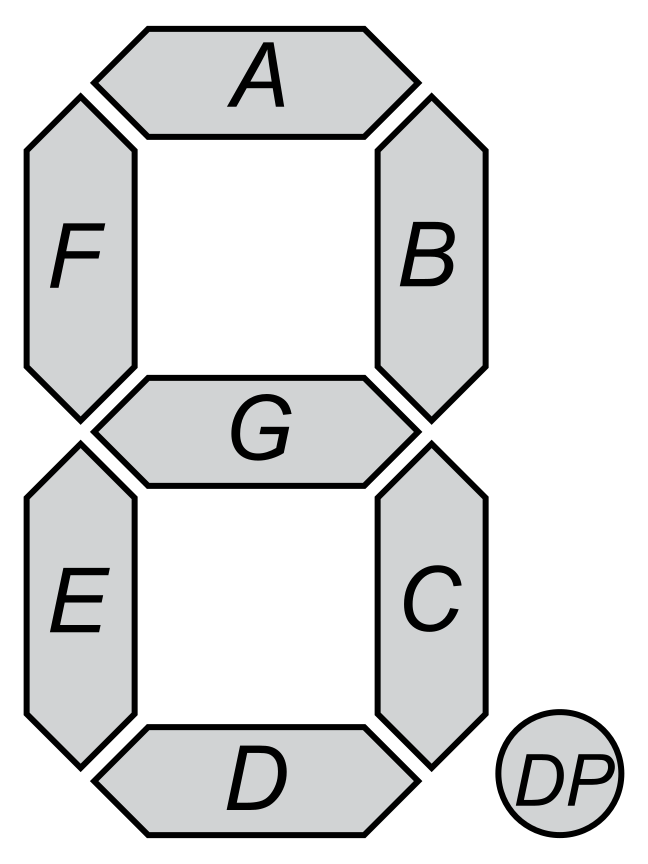
\includegraphics[scale = 0.1]{img/SevenSegDisplay.png}
    \caption{Segments d'un afficheur}
\end{figure}

Un afficheur sept segments est utilisé pour afficher des informations vers un utilisateur en allumant une partie des segments. Par exemple si on veut afficher le chiffre \textit{2}, on allume les segments \textit{A, B, D, E, G}.

\medskip

Faire la table de vérité de l'afficheur sept segments pour les chiffres allant de \textbf{0 à 15 en hexadécimal}

\medskip

Décrire l'entité et l'architecture votre table de vérité en VHDL.

\medskip

Simuler et vérifier le bon comportement de votre table de vérité

\medskip

Connecter les entrées de votre décodeur sept segments aux switchs (SW$x$) et les sorties aux afficheurs sept segments (HEX$x$) de la carte DE2. Tester et vérifier le bon fonctionnement.
\section{Logique séquentielle}
\subsection{Compteur}
\label{sec:BasicCnt}
Voici la table de vérité d'un simple compteur : 

\begin{table}[ht]
    \centering
    \begin{tabular}{c c c|c} 
        $ARst\_N$ & $Clk$ & $En$ & $Q_n$ \\ 
        \hline
        0 & * & * & 0 \\
        1 & \risingedge & 0 & $Q_{n-1}$ \\
        1 & \risingedge & 1 & $Q_{n-1} + 1$

    \end{tabular}
    \caption{Table de vérité d'un compteur}
    \label{ttab:BasicCnt}
\end{table}

Implémenter cette table de vérité en VHDL en utilisant un \textit{process} et \textbf{respectant bien la priorité}. Contraigner le vecteur $Q_n$ sur \textbf{8 bits}.

\medskip

Simuler votre compteur et vérifier que votre implémentation respecte bien la table de vérité.


\subsection{Cascade de compteurs}

Faire un compteur qui comptera toutes les secondes. Afficher la valeur de ce compteur sur un afficheur sept segments. Ce compteur devra compter 0 à 15.

\medskip

Faire un schéma fonctionnel en faisant apparaître deux compteurs en cascades. \\ 
\textbf{NB: Il est interdit de connecter aux entrées horloges autres que des signaux horloges}.

\medskip

Implémenter votre schéma fonctionnel en VHDL.

\medskip

A l'aide de l'analyseur logique (Signal Tap Logic Analyzer) visualiser le signal \textit{Q} des compteurs ainsi que le signal \textit{En} du second compteur. 

\medskip

Compiler, programmer et en utilisant l'analyseur logique, déclencher l'acquisition lorsque \textit{En} vaut $1$. Vérifier que \textit{En} est à $1$ que pendant un seul coup d'horloge.


\subsection{Machine à états}
Modéliser une machine a états qui permet d'incrémenter un compteur \textbf{d'une unité} lorsque l'on appuie sur un bouton.

\medskip

Créer le composant \textit{FsmBtn} et implémenter \textbf{uniquement} la machine à états.

\medskip

Valider le bon fonctionnement de votre machine à états en utilisant un compteur et en visualisant son contenu sur un afficheur sept segments. Utiliser le bouton \textit{KEY0} incrémenter le compteur.

\medskip

Sur le compteur de \ref{sec:BasicCnt}, ajouter le signal \textit{ud} qui permettra de changer la direction de comptage du compteur. Ce signal est le moins prioritaire de tous.

\medskip

Ajouter le nouveau signal à la table de vérité \ref{ttab:BasicCnt}.

\medskip

Valider le bon fonctionnement en simulation.

\medskip

En ajoutant une nouvelle instance du composant \textit{FsmBtn}, ajouter la fonctionnalité de décrémenter le compteur \textbf{d'une unité} lorsque l'on appuie sur un autre bouton. Utiliser le bouton \textit{KEY1} décrémenter le compteur.

\section{Mini projet - Horloge}

L'horloge n'affichera que les \textbf{heures} et les \textbf{minutes}. L'affichage des dizaine et unités des heures et des minutes se fera sur afficheur sept segments chacun.

\medskip

L'horloge aura deux modes de fonctionnement. Un mode normal où l'heure compte normalement et un mode configuration où on pourra venir modifier les heures et les minutes.

\medskip
Si on appuie sur \textit{KEY1}, on rentre en mode configuration.

\medskip 

Lorsque l'on appuie sur \textit{KEY2} ou \textit{KEY0}, on incrémentera ou décrémentera respectivement soit les heures soit les minutes.

\medskip

Lorsque l'on rentre en mode configuration, ce sont les minutes qui peuvent être modifies. Un nouvel appuie sur \textit{KEY1}, ce seront les heures qui pourront être modifies. Un nouvel appui sur \textit{KEY1}, on revient en mode normal.

\medskip

En utilisant les composants et en modélisant des nouveaux, faites un schema fonctionnel et les machines à états nécessaires pour modéliser l'horloge.

\medskip

Implémenter votre modélisation en VHDL.

\medskip

Valider votre implémentation en simulation.

\medskip

Valider votre implémentation sur votre carte.